%%%%%%%%%%%%%%%%%%%%%%%%%%%%%%%%%%%%%%%%%
% Short Sectioned Assignment
% LaTeX Template
% Version 1.0 (5/5/12)
%
% This template has been downloaded from:
% http://www.LaTeXTemplates.com
%
% Original author:
% Frits Wenneker (http://www.howtotex.com)
%
% License:
% CC BY-NC-SA 3.0 (http://creativecommons.org/licenses/by-nc-sa/3.0/)
%
%%%%%%%%%%%%%%%%%%%%%%%%%%%%%%%%%%%%%%%%%

%----------------------------------------------------------------------------------------
%	PACKAGES AND OTHER DOCUMENT CONFIGURATIONS
%----------------------------------------------------------------------------------------

\documentclass[paper=a4, fontsize=11pt]{scrartcl} % A4 paper and 11pt font size

\usepackage[T1]{fontenc} % Use 8-bit encoding that has 256 glyphs
\usepackage{fourier} % Use the Adobe Utopia font for the document - comment this line to return to the LaTeX default
\usepackage[english]{babel} % English language/hyphenation
\usepackage{amsmath,amsfonts,amsthm} % Math packages

\usepackage{lipsum} % Used for inserting dummy 'Lorem ipsum' text into the template

\usepackage{sectsty} % Allows customizing section commands
\allsectionsfont{\centering \normalfont\scshape} % Make all sections centered, the default font and small caps

\usepackage{fancyhdr} % Custom headers and footers
\pagestyle{fancyplain} % Makes all pages in the document conform to the custom headers and footers
\fancyhead{} % No page header - if you want one, create it in the same way as the footers below
\fancyfoot[L]{} % Empty left footer
\fancyfoot[C]{} % Empty center footer
\fancyfoot[R]{\thepage} % Page numbering for right footer
\renewcommand{\headrulewidth}{0pt} % Remove header underlines
\renewcommand{\footrulewidth}{0pt} % Remove footer underlines
\setlength{\headheight}{13.6pt} % Customize the height of the header

\numberwithin{equation}{section} % Number equations within sections (i.e. 1.1, 1.2, 2.1, 2.2 instead of 1, 2, 3, 4)
\numberwithin{figure}{section} % Number figures within sections (i.e. 1.1, 1.2, 2.1, 2.2 instead of 1, 2, 3, 4)
\numberwithin{table}{section} % Number tables within sections (i.e. 1.1, 1.2, 2.1, 2.2 instead of 1, 2, 3, 4)

\setlength\parindent{0pt} % Removes all indentation from paragraphs - comment this line for an assignment with lots of text

\usepackage{graphicx}
\graphicspath{ {./img/} }
\usepackage{float}

%----------------------------------------------------------------------------------------
%	TITLE SECTION
%----------------------------------------------------------------------------------------

\newcommand{\horrule}[1]{\rule{\linewidth}{#1}} % Create horizontal rule command with 1 argument of height

\title{	
\normalfont \normalsize 
\textsc{Department of Computer Science, University of Helsinki} \\ [25pt] % Your university, school and/or department name(s)
\horrule{0.5pt} \\[0.4cm] % Thin top horizontal rule
\huge Exercise2: Principal component analysis and factor analysis \\ % The assignment title
\horrule{2pt} \\[0.5cm] % Thick bottom horizontal rule
}

\author{Han Xiao} % Your name

\date{\normalsize\today} % Today's date or a custom date

\begin{document}

\maketitle % Print the title

%----------------------------------------------------------------------------------------
%	PROBLEM 1
%----------------------------------------------------------------------------------------

\section{Question 1}

The projected data (blue circle) points in this figure are projections of the original data points onto the first and second principal components. For example, the value of some data point, $x$, on the x axis is the projection of $x$ onto the first principal component, denoted as $u_1$. The projection operation is $x \cdot u_1^{'}$. In the data compression sense, they can be seen as the compressed data using the first and second principal components. The compressed data can later be used to approximately reconstruct the original data. \newline

The five red lines represent the original five variables respectively. The direction, $(x, y)$ of each line can be understood as the {\em relative} ratio that the corresponding variable incorporates the direction of the first principle component {\em against} the second principle component respectively. For example, if a variable has relative larger x value than y value, the variable can be seen to be more like to the first principle component and vice versa. The length of line can be seen as the {\em overall} degree that the corresponding variable incorporates the two principle components. If the length is short, then we can infer that the variable doesn't have a strong relationship with the two components.

\begin{figure}[H]
  \centering
  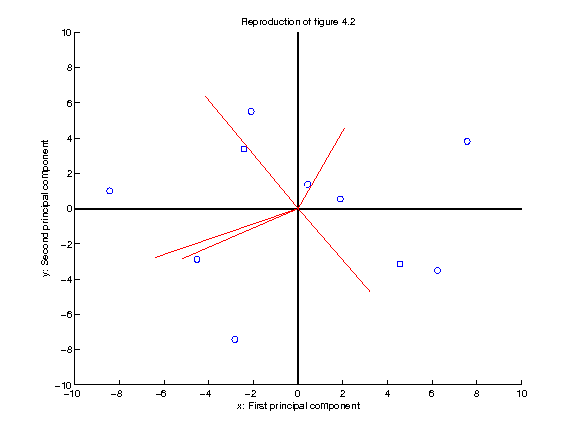
\includegraphics[scale=.7]{reproduct42}
  \caption{Reproduction of figure 4.2 on page 34 of the lecture notes}
\end{figure}


%------------------------------------------------


%----------------------------------------------------------------------------------------
%	PROBLEM 2
%----------------------------------------------------------------------------------------

\section{Question 2}

I sort the eigen values in descending order and got the following figure:

\begin{figure}[H]
  \centering
  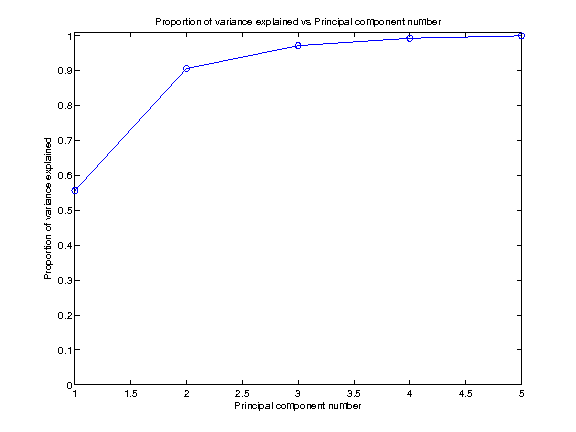
\includegraphics[scale=.7]{variance_explained}
  \caption{Proportion of variance explained vs number of principal component used}
\end{figure}

  
%----------------------------------------------------------------------------------------
%	PROBLEM 3
%----------------------------------------------------------------------------------------

\section {Question 3}

One key note about this question is the partial direvative of $J_{rot} (U)$, given $A$ is of size $n \times m$ and $U$ of size $m \times m$.

\[ \frac {\partial} {\partial U_{nm}} J_{rot } (U) = 4 \sum\limits_i^n (\sum\limits_k^m A_{ik} U_{km})^3\]

Constrained by orthonormality, after each iteration of gradient descent, 

\[U=(W W^T)^{-\frac {1} {2}}W \]

%----------------------------------------------------------------------------------------
%	PROBLEM 4
%----------------------------------------------------------------------------------------

\section {Question 4}

Indeed it does give me the result as in the lecture notes! The $J_{rot}$ decreases as plotted in the following figure:

\begin{figure}[H]
  \centering
  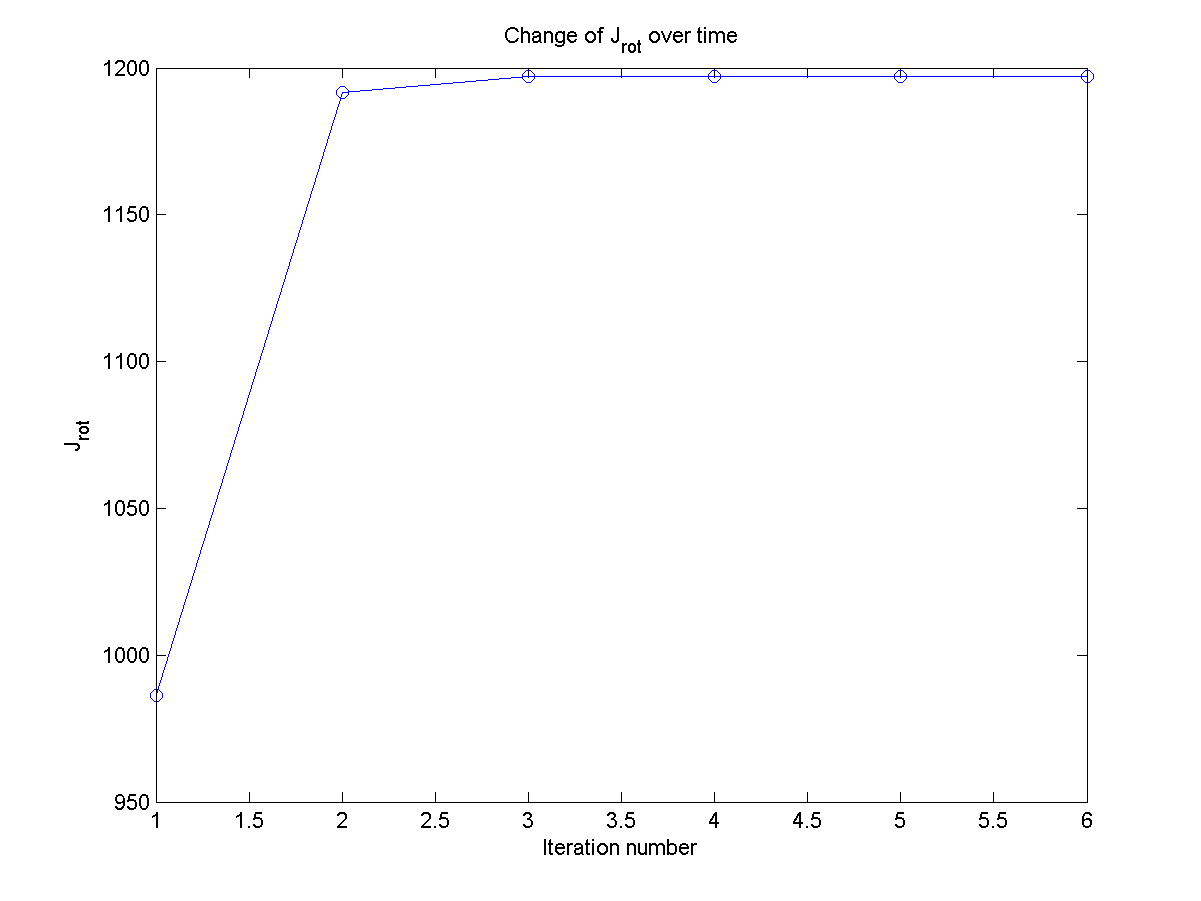
\includegraphics[scale=.7]{J_rot}
  \caption{$J_{rot}$ as iteration process goes on}
\end{figure}

%----------------------------------------------------------------------------------------
%	PROBLEM 5
%----------------------------------------------------------------------------------------

\section {Question 5}

The data points in the figure are the projection of actual data points onto the two factors.

The direction of the five lines, each representing one variable, denotes the proportion that the two factors accounts for the variable, while the length of the line denotes how many they as a whole account for the variable.

Note: the figure is flipped compared to the lecture note figure.

\begin{figure}[H]
  \centering
  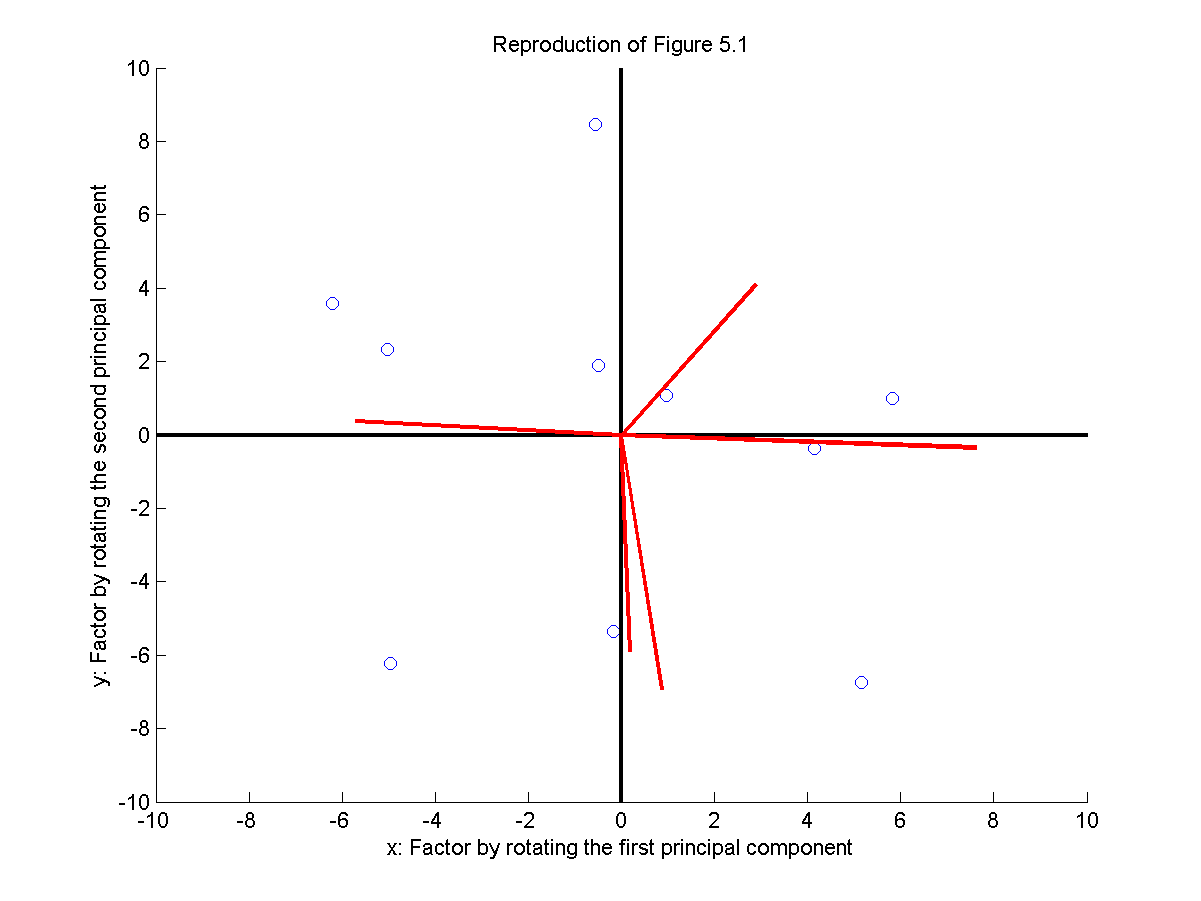
\includegraphics[scale=.7]{reproduct51}
  \caption{Reproduction of figure 5.1}
\end{figure}

\end{document}
